\chapter{Realization}
\label{ch:setup}


\section{Realization of the real data recording system}

\subsection{Hardware for the recordings}
To record real data that suits our baseline, we must design a system to record and save lots of data. As we had the opportunity to place it on the HEIA-FR, we decided to design a system containing an embedded system, two microphones, a camera, and an embedded system. For the hardware, we chose to ensure that the system is easily replicable and that the system is not too expensive. We used hardware available at the HEIA and Rosas. The system design is shown in Figure \ref{fig:real_data_recording_system}.

The HEIA-FR has a small balcony on the 4th floor with hardware installed for other projects. We used this balcony to install our system. The balcony is located on the side of a street and has a barrier on which we can attach hardware to have a good view of the street. 

To record real data that suits our baseline, we must get hardware to record and save the data. The hardware we used is the following:

\paragraph{Microphones}
We used two microphones to record the sound. We used the \textit{nsrt mk3 dev kit} from \textit{convergenceinstruments} \footnote{\url{https://convergenceinstruments.com/}} with the USB audio interface (Figure \ref{fig:nsrt_mk3_mic}). Prof. Marc-Antoine Fénart chose the microphones himself. We used two microphones to have a stereo sound recording.

\begin{figure}[H]
    \centering
    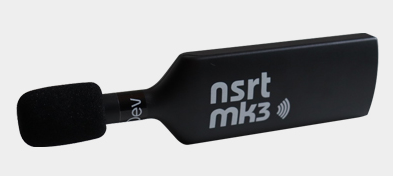
\includegraphics[width=.5\textwidth]{images/nsrt_mk3_mic.png}
    \caption{Microphone used for the recordings}
    \label{fig:nsrt_mk3_mic}
\end{figure}

\paragraph{Camera}
The camera used is a webcam from Rosas that was available at the moment of the installation. We used the \textit{C310 webcam} from \textit{logitech} \footnote{\url{https://www.logitech.fr/fr-fr/product/hd-pro-webcam-c920}} since it meets our needs (Figure \ref{fig:c310_webcam}). 

\begin{figure}[H]
    \centering
    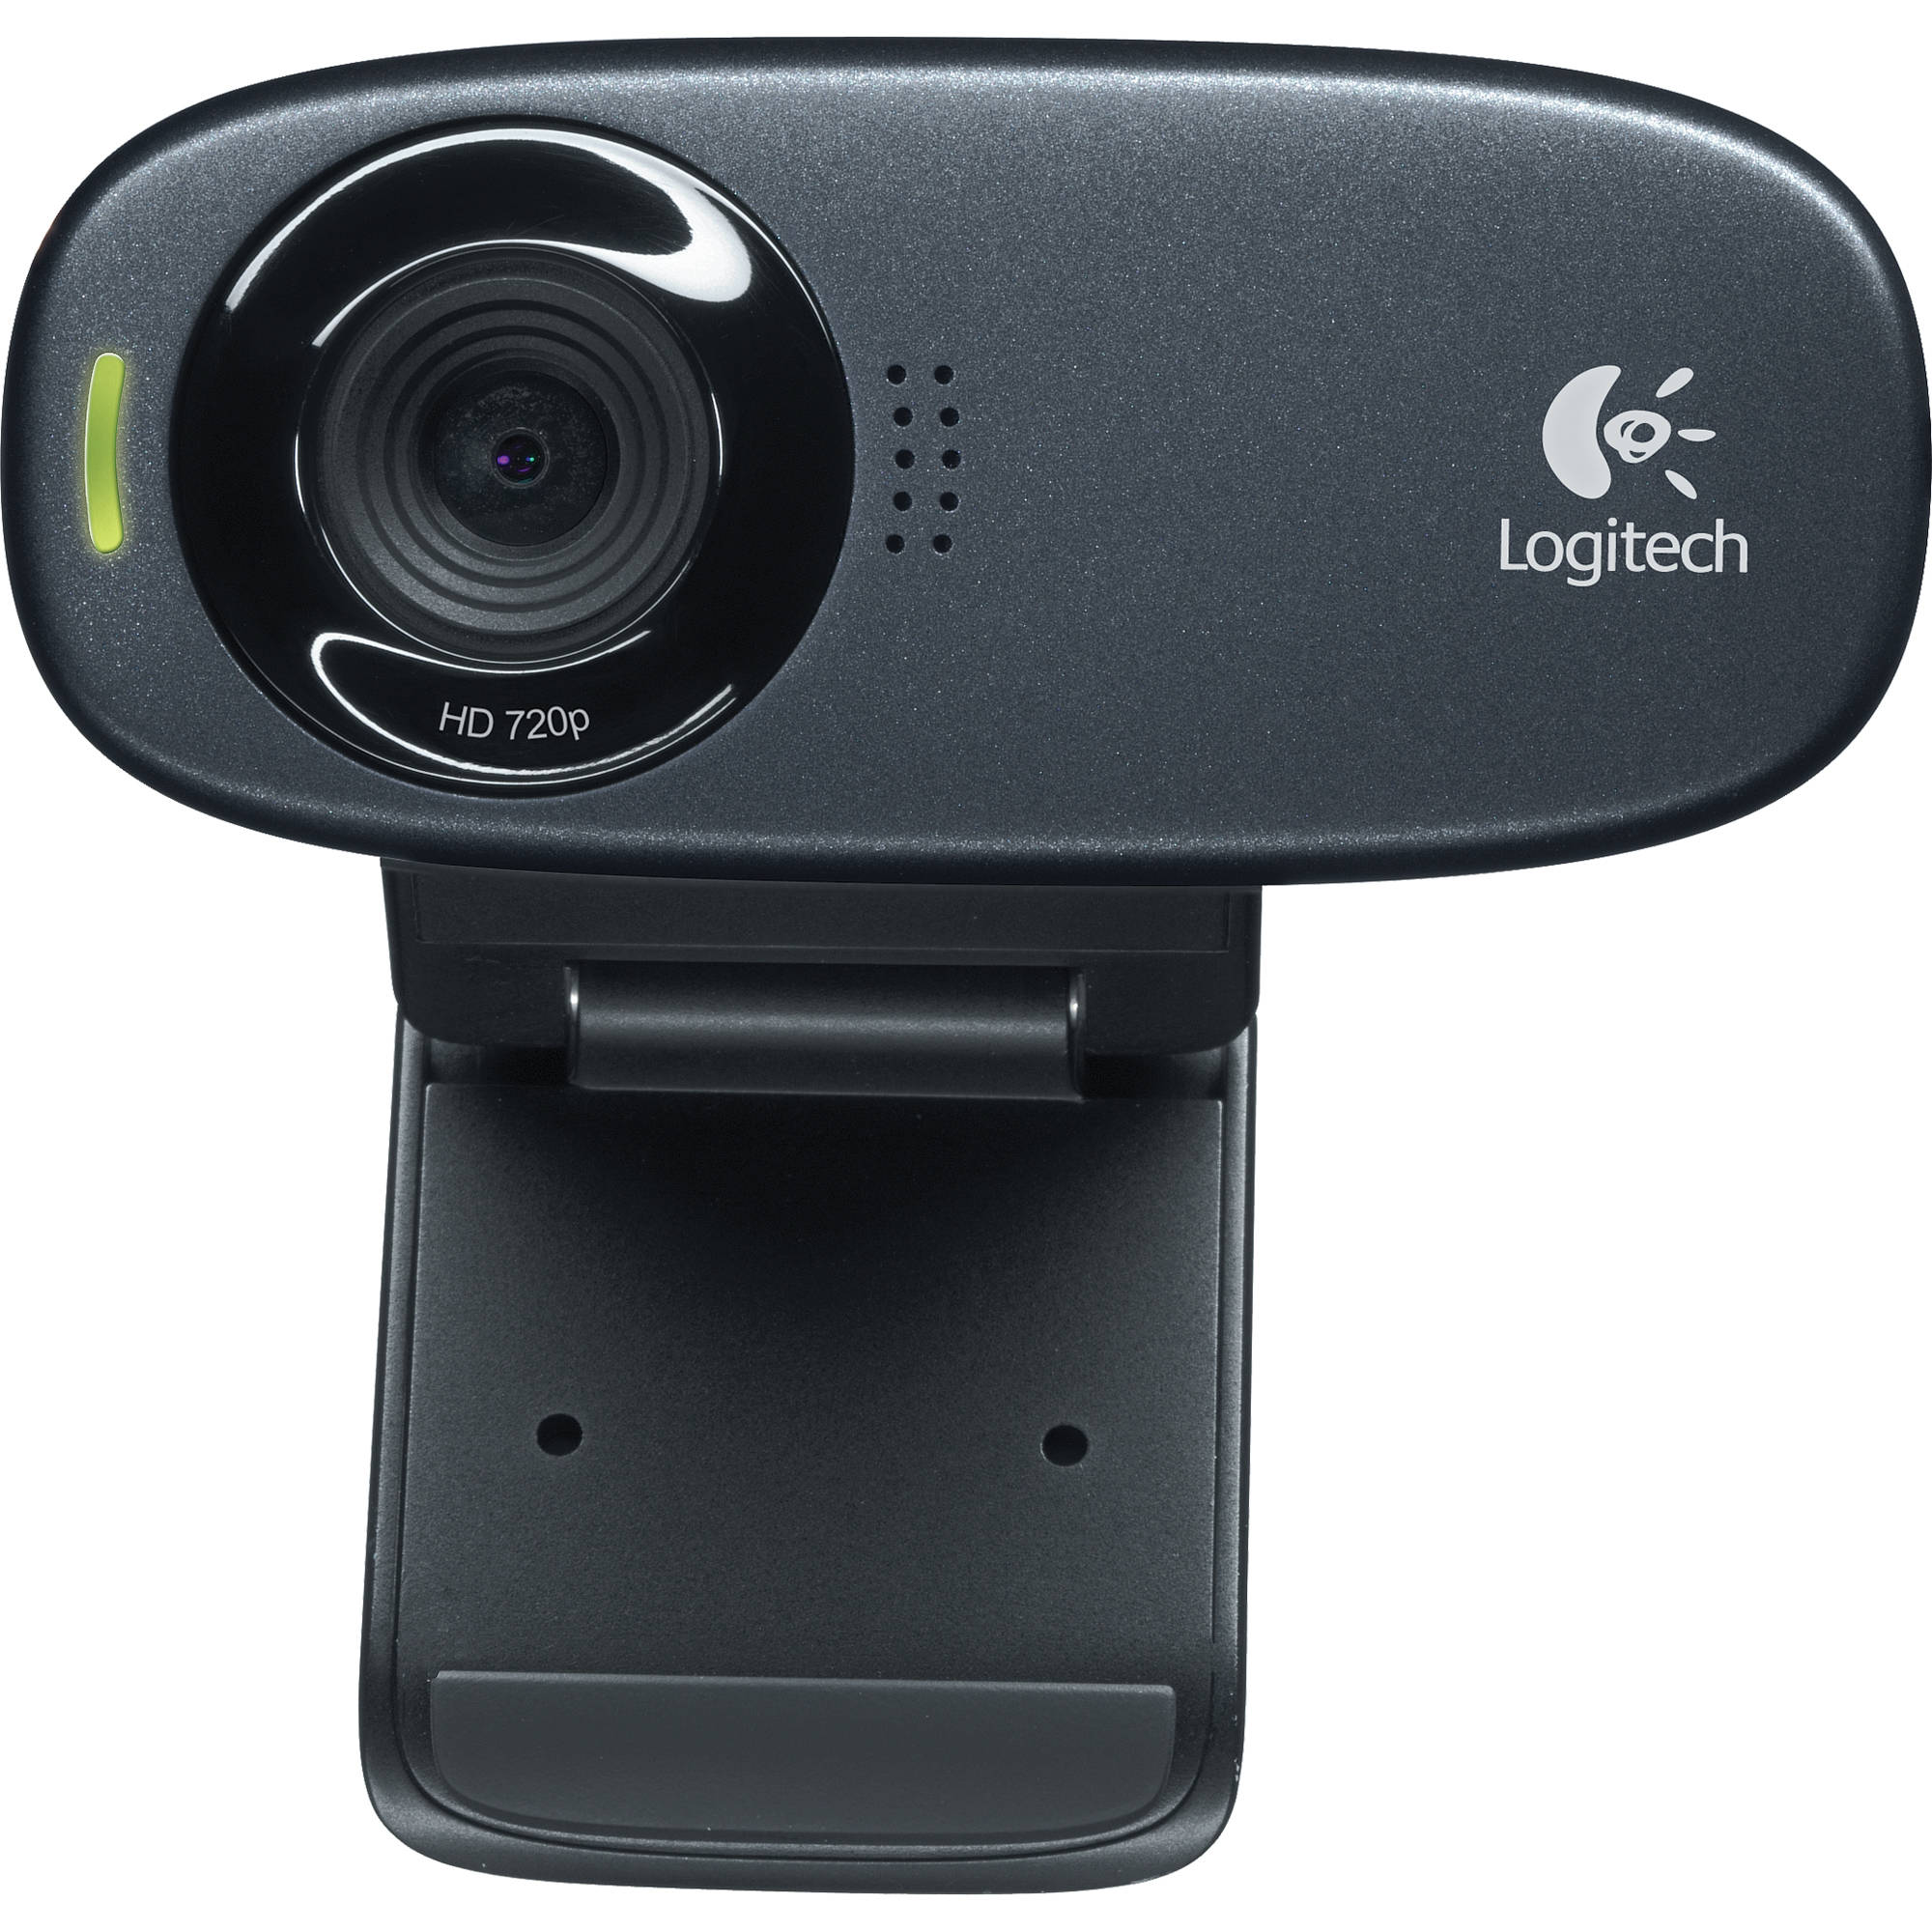
\includegraphics[width=.5\textwidth]{images/c310_webcam.png}
    \caption{Webcam used for the recordings}
    \label{fig:c310_webcam}
\end{figure}

\paragraph{Embedded system}
We used the \textit{Raspberry Pi 4} from \textit{raspberrypi} \footnote{\url{https://www.raspberrypi.org/products/raspberry-pi-4-model-b/}} as an embedded system (Figure \ref{fig:raspberry_pi_4}). We used this embedded system because it is powerful enough to run the recordings and was available at the HEIA-FR. Since our microphones and our camera have USB connectors, we needed an embedded system with at least 3 USB connectors.

\begin{figure}[H]
    \centering
    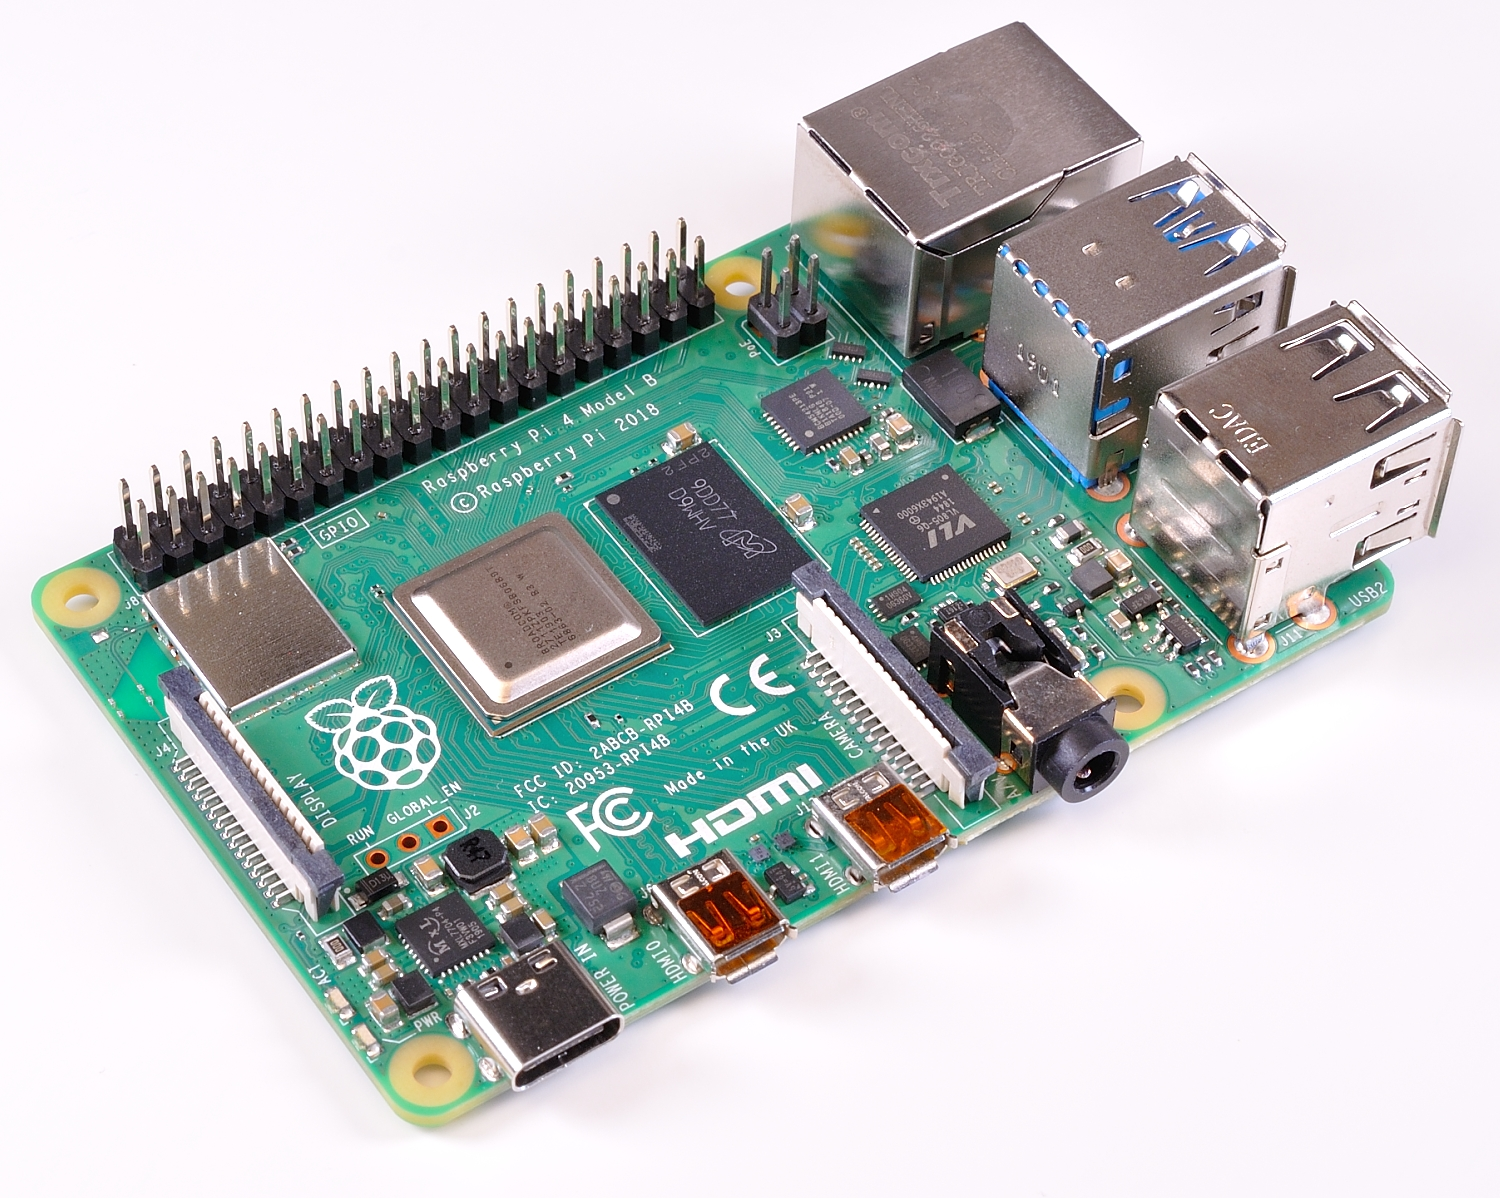
\includegraphics[width=.5\textwidth]{images/raspberry_pi_4.png}
    \caption{Raspberry Pi 4 used for the recordings}
    \label{fig:raspberry_pi_4}
\end{figure}

\paragraph{Storage}

We asked the HEIA-FR for a storage server in the school to upload the data. They lend us a server with two terabyte of storage accessible from the school network and from the internet.

\paragraph{Data transmission}

Since there is no network cable on the HEIA-FR's balcony, we used a 4G modem lent by the school to transmit the data to the storage server. We used a 4G LTE N300 router from D-Link \footnote{\url{https://eu.dlink.com/}} (Figure \ref{fig:4g_lte_router}) to transmit the data. We used a SIM card from Swisscom, also lent by the school to transmit the recordings via the Internet.

\begin{figure}[H]
    \centering
    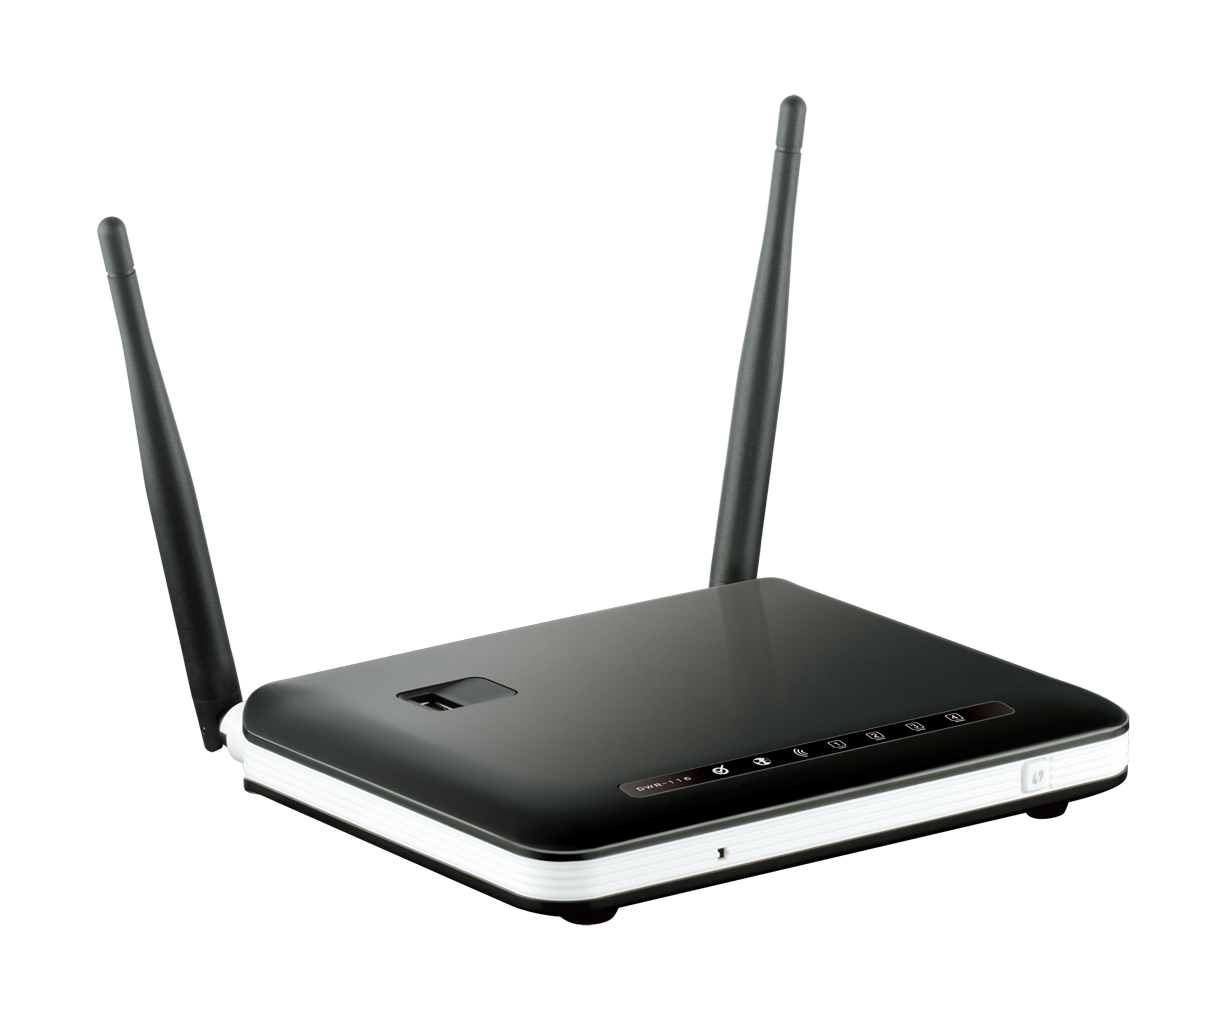
\includegraphics[width=.5\textwidth]{images/4g_lte_router.png}
    \caption{D-Link router used for the recordings}
    \label{fig:4g_lte_router}
\end{figure}

\paragraph{3D support}

To attach the microphones, we designed 3D pieces with CAD software to 3D print them. We used \textit{tinkercad} to design the pieces. After the design, we could give the 3D models to the mechanics at ROSAS to 3D print them. The 3D pieces are shown in Figure \ref{fig:3d_pieces}.

\begin{figure}[H]
    \centering
    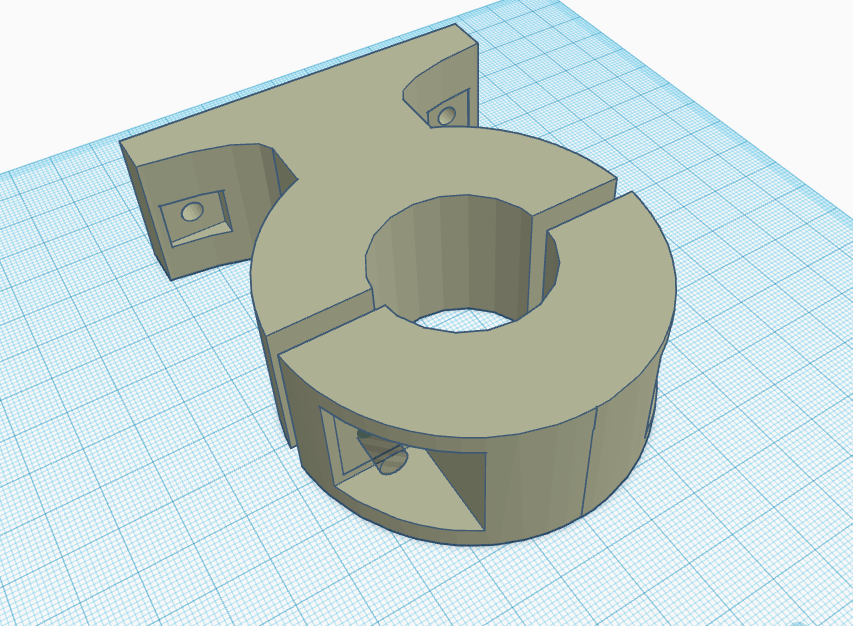
\includegraphics[width=.5\textwidth]{../Images/tinkercad_mic_support.png}
    \caption{3D pieces}
    \label{fig:3d_pieces}
\end{figure}

% TODO ajouter images
We can see the installed hardware in Figure TODO Ajouter image !

\subsection{Software for the recordings}

To record the data, we must have software to control the hardware. We must also have software to transmit the data to the storage server. This subsection describes the software used to make the system work.

\paragraph{Operating system}

We used \textit{Raspberry Pi OS} \footnote{\url{https://www.raspberrypi.org/software/operating-systems/}} as the operating system for the Raspberry Pi because it is the official operating system for the Raspberry Pi, and it also is the most used operating system for the Raspberry Pi. It is based on \textit{Debian} \footnote{\url{https://www.debian.org/}} and is optimized for the Raspberry Pi. It is also easy to install and use.

\paragraph{Audio recording}

Since each microphone has its sound card, we must treat them as one sound card per microphone on the operating system. This can cause some issues if we start the recording at a slightly different time. This problem can, for example, be the case when we execute two consecutive commands, one after the other, in a script to start the microphone recording. We can use \textit{Advanced Linux Sound Architecture (ALSA)} \footnote{\url{https://www.alsa-project.org/}} to manage each sound interface and combine them into one virtual sound interface to be able to start the record from both sound cards at the same time. This can be done in a configuration file for ALSA. We used the following configuration file to combine the two sound cards into one virtual sound card:

\begin{lstlisting}[language=bash]
pcm.mic1 {
  type hw
  card NSRTmk3Dev
  device 0
}

pcm.mic2 {
  type hw
  card NSRTmk3Dev_1
  device 0
}

pcm.mic12 {
  type multi
  slaves.a.pcm mic1
  slaves.a.channels 1
  slaves.b.pcm mic2
  slaves.b.channels 1
  bindings.0.slave a
  bindings.0.channel 0
  bindings.1.slave b
  bindings.1.channel 0
}
\end{lstlisting}

This configuration file will create a virtual sound card called mic12 that will combine the two sound cards: \textit{mic1} and \textit{mic2}. We can then use this virtual sound card to start the recording on both sound cards simultaneously.

\paragraph{video recording and synchronization}

We use \textit{ffmpeg} \footnote{\url{https://www.ffmpeg.org/}} to record the video and the audio synchronously. The command used to record the video and the audio is the following:

\begin{lstlisting}[language=bash]
    ffmpeg -f alsa -thread_queue_size 2048 -i plug:mic12 -f v4l2 -thread_queue_size 2048 -input_format mjpeg -video_size 600x400 -i /dev/video0 -c:a aac -map 0:a -map 1:v -segment_time 00:10:00 -f segment /mnt/videos/$current_date/output%05d.mp4
\end{lstlisting}

This command combines the video from the device \textit{/dev/video0} and the virtual sound card \textit{mic12} in a single file containing audio and video.

Before installing the system on the HEIA-FR balcony, we calculated the delay between the video and the audio by clapping in front of the webcam and the microphones. Since the delay found was inferior to 100 milliseconds and we only recorded the video to provide ground truth in a 2 seconds period, we admitted it was negligible for the dataset annotation task.

\paragraph{Raspberry pi access for administration}

We used a server from the HEIA-FR to store the data. We can access the server through OpenSSH on the local network of the HEIA-FR.

Since we don't want to go to the HEIA-FR every time we want to access the Raspberry Pi, and we don't want to have ports open on the internet, we use \textit{remote.it} \footnote{\url{https://remote.it/}} to access the Raspberry Pi remotely. \textit{Remote.it} is a service that allows us to access the Raspberry Pi remotely without opening ports on the internet. It creates a VPN between the Raspberry Pi and the \textit{remote.it} server and gives us the VPN address on the \textit{remote.it} web application. We can then access the Raspberry Pi through the VPN.


\paragraph{Data transmission}

Since the data we transmit could be sensitive, we transferred it using a secure file transfer protocol. SFTP is a network protocol that provides file access, file transfer, and file management functionalities over a secure channel. We used \textit{OpenSSH} \footnote{\url{https://www.openssh.com/}} to transfer the data. OpenSSH is a suite of secure networking utilities based on the Secure Shell (SSH) protocol. OpenSSH encrypts all traffic (including passwords) to eliminate eavesdropping, connection hijacking, and other attacks. To transfer the data, we mounted the storage server as a local drive on the Raspberry Pi by using the following command:

\begin{lstlisting}[language=bash]
    sshfs drosset@proxy51.rt3.io:/home/drosset/workspace/videos /mnt/videos -p 33838
\end{lstlisting}

This command will ask for a password to connect to the server and provide us with a local drive on the Raspberry Pi that is connected to the server. We can then use this local drive to store the data directly on the storage server.

The global architecture of the system is shown in Figure \ref{fig:global_architecture}. This diagram helps us understand how each system component is connected and how to access them.

\begin{figure}[H]
    \centering
    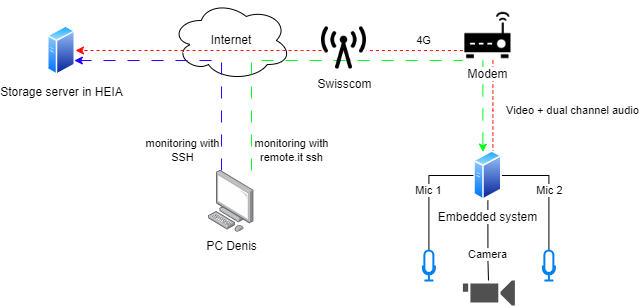
\includegraphics[width=1\textwidth]{../Images/real_data_recording_system.drawio.png}
    \caption{Global architecture}
    \label{fig:global_architecture}
\end{figure}



\section{Dataset creation}

For most of the dataset management, we used Python. Python is a programming language that gives us many dataset management tools. We used Python to split the recordings into smaller files, annotate the dataset, and manage the folders.

Once we set up the hardware and the software allows us to record the vehicles on the street, we can build a dataset. The recordings of the vehicles contain audio and video in mp4 files of ten minutes each. We must split the recordings into smaller files to get to the two seconds of length defined in section \ref{sec:vehicle_recordings}. We split the recordings into two seconds files. Since splitting a video can be time-consuming, we launch it in a subprocess to execute it concurrently on multiple files at the same time. We used the following script:

\begin{lstlisting}[language=python]
for file in files:
    subprocess.call(['ffmpeg', '-i', directory + '/' + file, '-c:v', 'libx264', '-crf', '22', '-map', '0', '-segment_time', time, '-reset_timestamps', '1', '-g', '30', '-sc_threshold', '0', '-force_key_frames', 'expr:gte(t,n_forced*'+str(time)+')', '-f', 'segment', directory[:-1]+'-2sec/' + file + '%05d.mp4'])
\end{lstlisting}

This script allows to have two seconds of video clips of the vehicles. We can then annotate the dataset.

\subsection{Dataset annotation}

A good practice when creating a dataset to classify it is to put the files in folders. Each folder represents a class. In our case, we use the classes defined in section \ref{sec:dataset_conception}: 

\begin{itemize}
    \item  \textit{left\_to\_right}: \textbf{D} The vehicle goes from the left to the right of the microphone.
    \item  \textit{right\_to\_left}: \textbf{A} The vehicle goes from the right to the left of the microphone.
    \item  \textit{no\_cars}: \textbf{S} No vehicles pass by the microphone.
    \item  \textit{multiple\_cars}: \textbf{W} Multiple vehicles pass by the microphone.
\end{itemize}

Each class has its folder. We can then annotate the dataset by moving the files to the correct folder. We developed a tool to annotate the dataset. The tool is an application that shows a 2-second video from the recordings. The user can then press a key in the application to automatically move the video to the class folder. The user can also press a "cancel" key to remove the last annotated video if the user makes a mistake. Figure \ref{fig:dataset_annotation_tool} (a) shows an example of the tool. We can see multiple vehicles in this video. The user can press the \textbf{W} key. In Figure \ref{fig:dataset_annotation_tool} (b), we see only one vehicle going from right to left. The user can then press the \textbf{D} key to save the file in the correct folder.

\begin{figure}[H]
    \centering
    \subfloat[\centering Multiple car]{{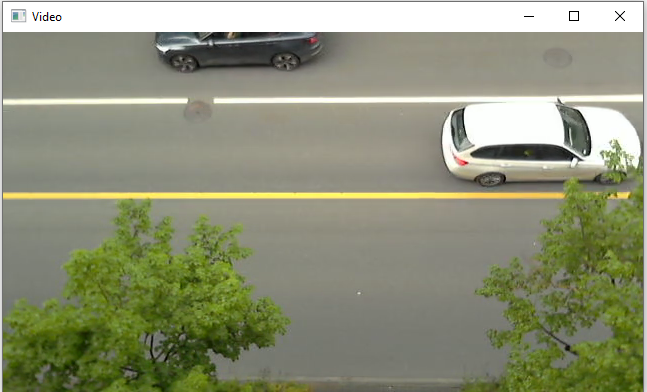
\includegraphics[width=4cm]{../Images/dataset_annotation_tool_multiple.png} }}%
    \qquad
    \subfloat[\centering Left to right]{{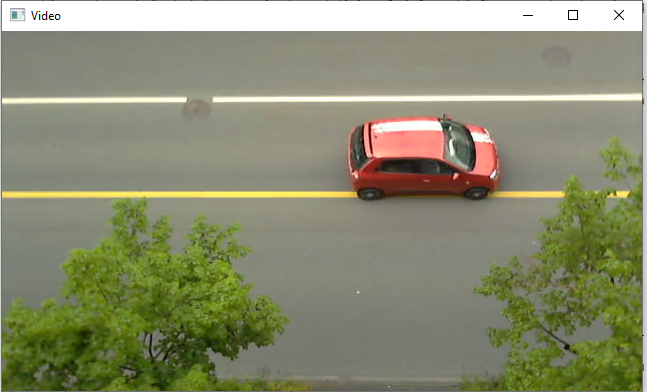
\includegraphics[width=4cm]{../Images/dataset_annotation_tool_left_to_right.png} }}%
    \caption{Dataset annotation tool}
    \label{fig:dataset_annotation_tool}
\end{figure}

Since the videos only show vehicles moving on a road, we don't need to play the video at real speed. The tool plays the video accelerated to gain time when annotating the dataset. 

\subsection{Dataset}

The annotation was done for 2037 videos and defines our baseline dataset for the project. The dataset contains 2037 videos of two seconds each. The dataset is split into four classes. The statistics for the classes are the following:

\begin{lstlisting}[language=bash]
classes:  ['left_to_right', 'multiple_cars', 'no_car', 'right_to_left']
total files:  2037
total files for class left_to_right:  513
total files for class multiple_cars:  234
total files for class no_car:  582
total files for class right_to_left:  708
\end{lstlisting}

We represent the statistics as a table in Table \ref{tab:dataset_statistics}.

\begin{table}[H]
    \centering
    \begin{tabular}{|c|c|}
        \hline
        \textbf{Class} & \textbf{Number of files} \\
        \hline
        left\_to\_right & 513 \\
        \hline
        multiple\_cars & 234 \\
        \hline
        no\_car & 582 \\
        \hline
        right\_to\_left & 708 \\
        \hline
    \end{tabular}
    \caption{Dataset statistics}
    \label{tab:dataset_statistics}
\end{table}

\subsection{Dataset annotation from audio}

Since the project aims to use audio to annotate the dataset, we also create a dataset from the audio. We can use the same tool to annotate the dataset. The tool plays the audio of the video instead of the video. The user can then press the same keys to annotate the dataset. Since we use two microphones, we can play the audio in a stereo headset to have all audio channels listenable during the annotation. We can then compare the results of the dataset annotated from the audio only with the results of the neural network trained on the dataset annotated from the video. 

\section{Neural Network for Sound Source Localization}

Once we have annotated the dataset, we can load it. We use the \textit{PyTorch} \footnote{\url{https://pytorch.org/}} library for the whole neural network process because it is popular, open-source, and free. It also has a lot of documentation. 

\subsection{Data preparation}



\subsection{Neural Network architecture}



\subsection{Training}


\section{Simulation model creation}

\subsection{Microsoft Project plugin}

\subsection{Unity plugin}

\subsection{Unity simulation creation}

The simulation is also faster than recording the data. We can generate a lot of data in a short time. The simulation is also cheaper than recording the data. We don't need to buy a vehicle and a camera to generate the data. We only need to buy a microphone and a speaker. The simulation is also more flexible than recording the data. We can change the position of the microphone and the camera easily. We can also change the vehicle's speed and the number of vehicles in the simulation. The simulation is also more reproducible than recording the data. We can generate the same data multiple times. We can also generate data for the same position of the sound source multiple times. The simulation is also more scalable than recording the data. We can generate data for any position of the sound source. We can also generate data for any number of vehicles. The simulation is also more controllable than recording the data. We can control the position of the sound source, the vehicle's speed, and the number of vehicles. The simulation is also more secure than recording the data. We can generate data without any risk of accidents. The simulation is also more accessible than recording the data. We can generate data without

\section{Adversarial Attack}

\subsection{Fast Gradient Signed Method implementation}

